\clearpage
\appendix
\section{Additional Figures}

\begin{figure}[h]
  \centering
  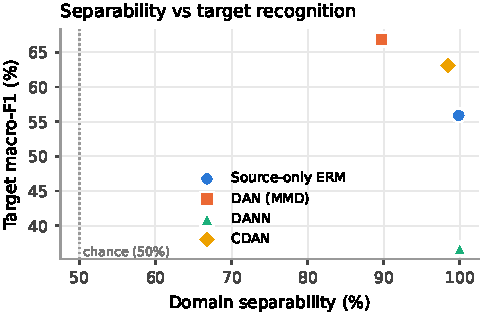
\includegraphics[width=0.5\textwidth]{figures/task2/fig3_separability.pdf}
  \caption{Target macro-F1 against source-vs-target separability for the four Task 2 methods; the dotted line marks chance (50\%).}
  \label{fig:task2_separability}
\end{figure}

\begin{figure}[h]
  \centering
  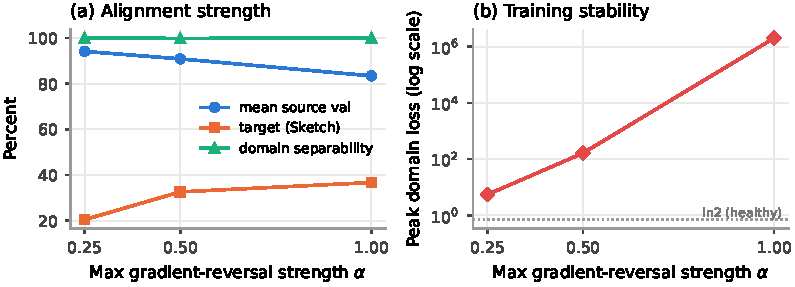
\includegraphics[width=0.72\textwidth]{figures/task2/fig5_alignment_study.pdf}
  \caption{DANN with $\alpha_{\max}\in\{0.25,0.5,1\}$: source macro-F1, target macro-F1 and separability, with the ERM target macro-F1 for reference.}
  \label{fig:task2_alignment_study}
\end{figure}

\begin{figure}[h]
  \centering
  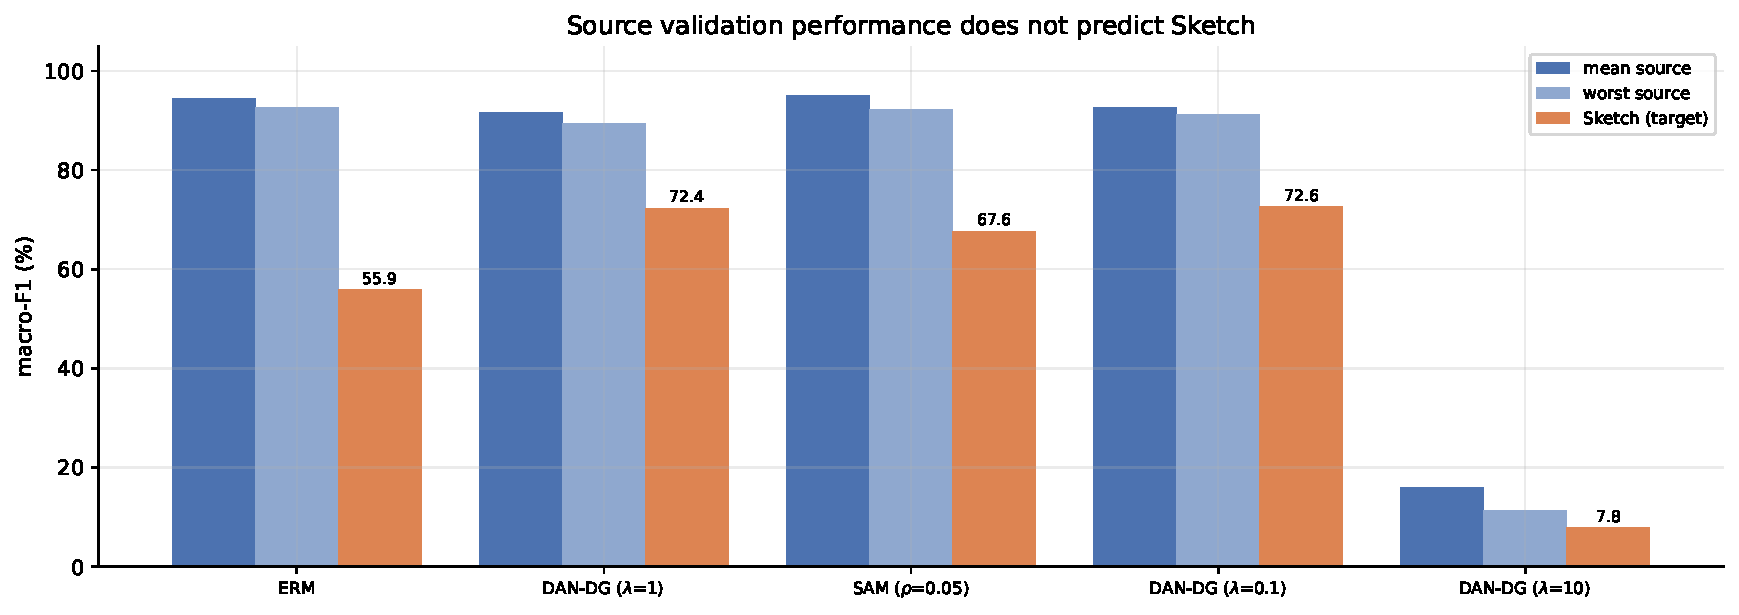
\includegraphics[width=\textwidth]{figures/task3/fig2_method_comparison.pdf}
  \caption{Mean-source, worst-source and Sketch macro-F1 for all Task 3 models.}
  \label{fig:task3_method_comparison}
\end{figure}

\begin{figure}[h]
  \centering
  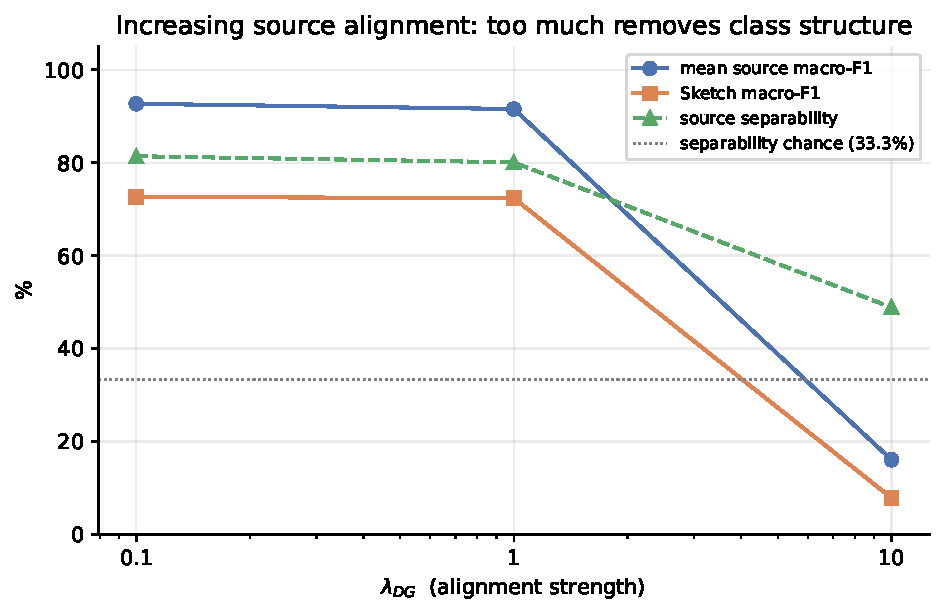
\includegraphics[width=0.62\textwidth]{figures/task3/fig3_alignment_study.pdf}\\[4pt]
  
\includegraphics[width=\textwidth]{figures/task3/fig4_per_class.pdf}
  \caption{Top: $\lambda_{\mathrm{DG}}$ study (mean source macro-F1, Sketch macro-F1, source separability; dotted line is chance). Bottom: per-class Sketch accuracy change against ERM.}
  \label{fig:task3_alignment}
\end{figure}

\begin{figure}[h]
  \centering
  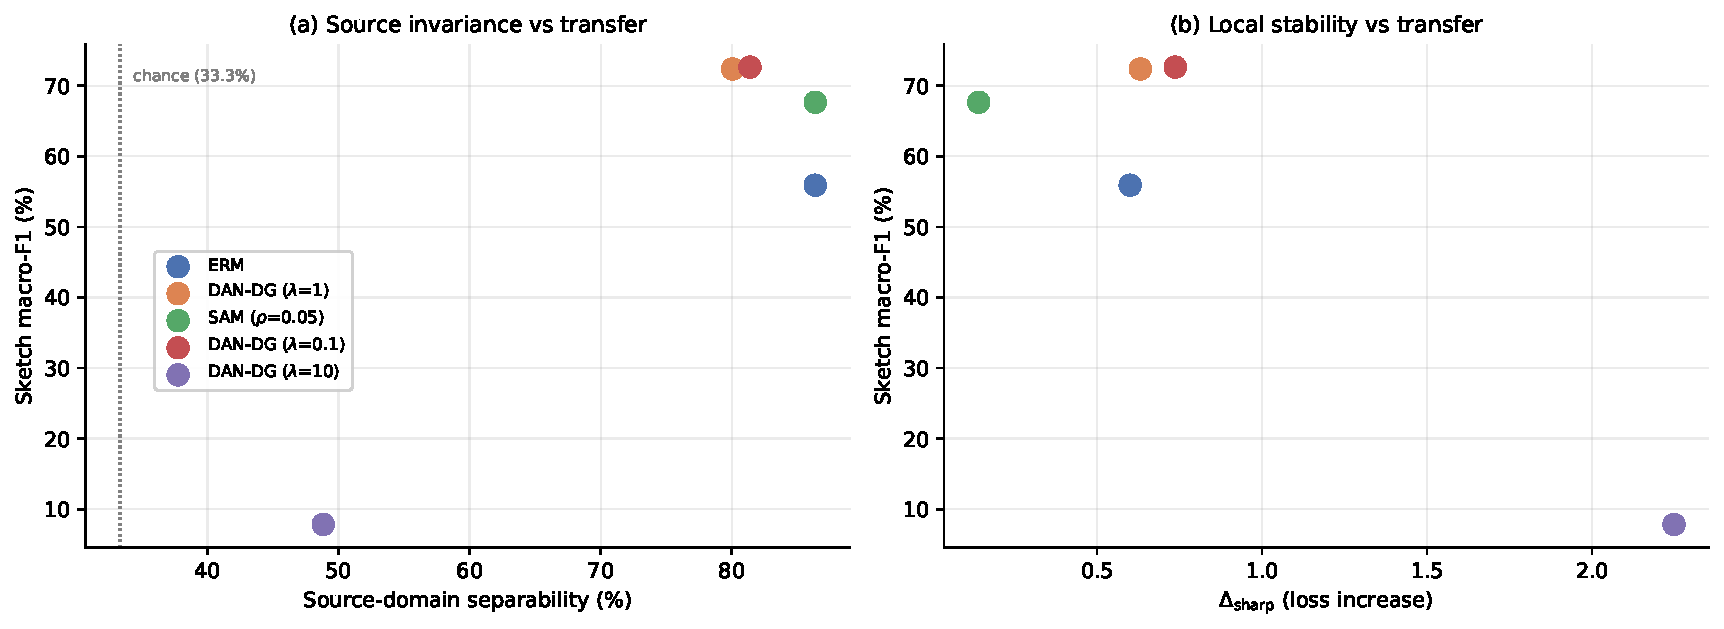
\includegraphics[width=\textwidth]{figures/task3/fig5_diagnostics.pdf}
  \caption{Sketch macro-F1 against (a) source-domain separability and (b) the sharpness proxy $\Delta_{\mathrm{sharp}}$.}
  \label{fig:task3_diagnostics}
\end{figure}

\begin{figure}[h]
  \centering
  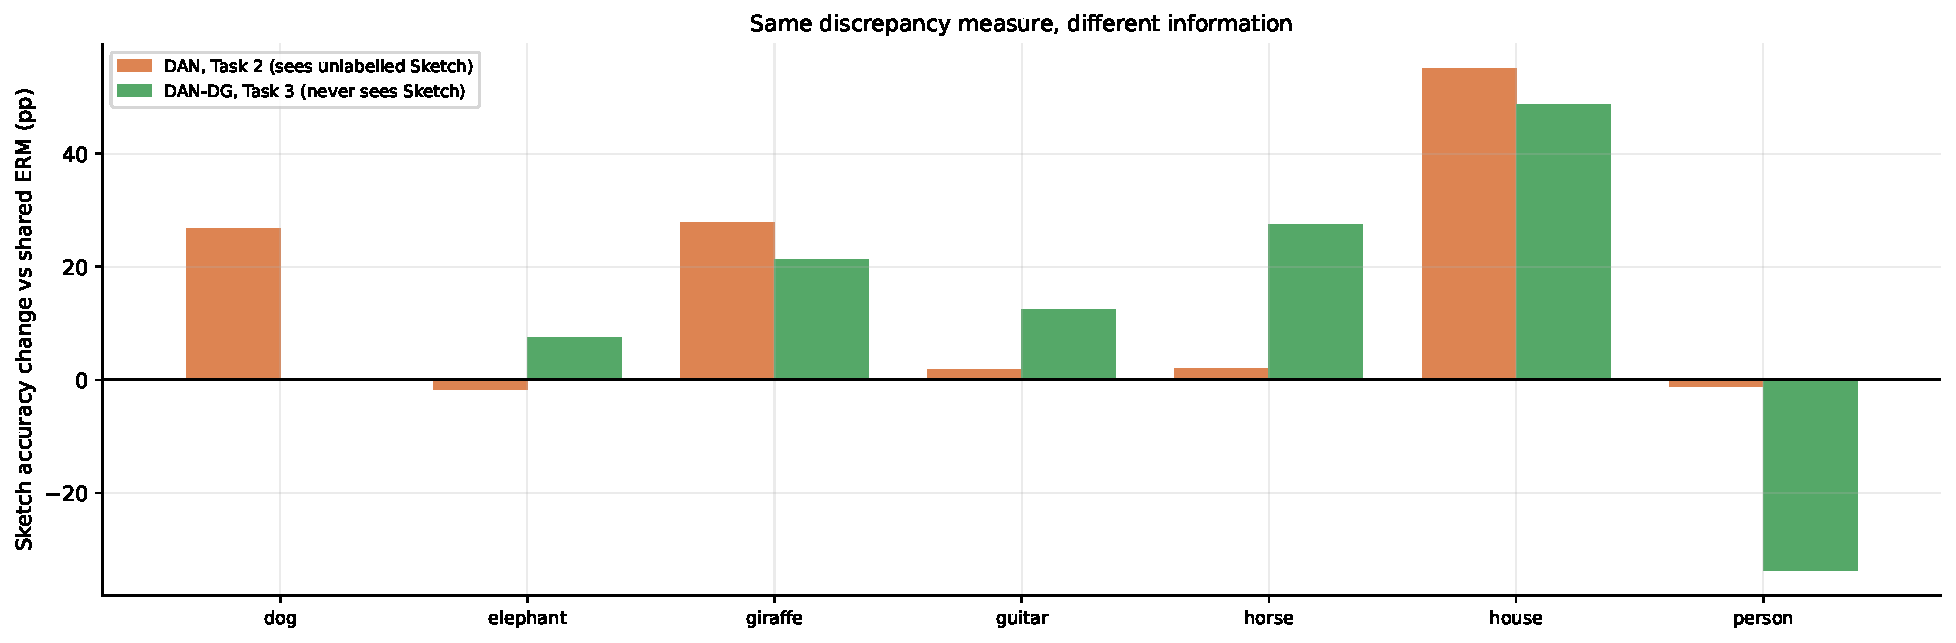
\includegraphics[width=\textwidth]{figures/task3/fig7_per_class_vs_task2.pdf}
  \caption{Per-class Sketch accuracy change against the shared ERM for DAN (Task 2) and DAN-DG (Task 3).}
  \label{fig:task3_vs_task2}
\end{figure}

\begin{figure}[h]
  \centering
  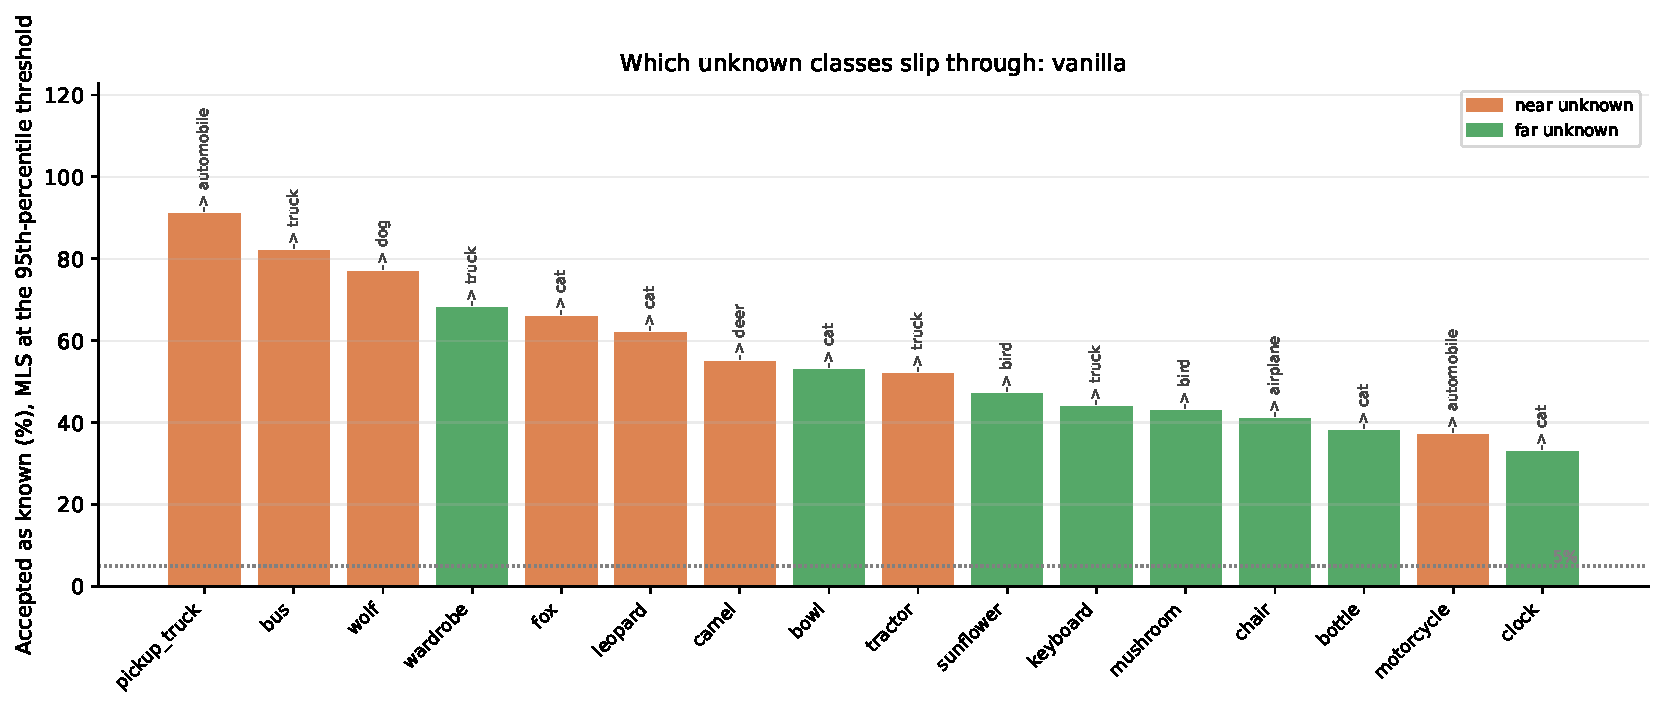
\includegraphics[width=\textwidth]{figures/task4/fig2_unknown_classes.pdf}
  \caption{Share of each unknown class accepted by Vanilla under MLS, annotated with the absorbing CIFAR-10 class (100 images per class).}
  \label{fig:task4_unknown_classes}
\end{figure}
